\documentclass{beamer}
\usetheme{Madrid}
\usefonttheme{professionalfonts}
\usecolortheme{rose}
\usepackage{fontspec}
\setmainfont{Times New Roman}
\usepackage{amsmath}
\usepackage{bm}
\usepackage{tikz}
\usepackage{svg}
\usepackage{graphics}
\usepackage{appendixnumberbeamer}
\usepackage{mathtools}
\usepackage{enumitem}
\usepackage[most]{tcolorbox}
\tcbset{
  thickitembox/.style={
    colback=white,
    colframe=white,
    left=2mm,
    before skip=4pt,
    after skip=4pt,
    borderline west={3pt}{0pt}{gray},  % ← 这里控制线条粗细和颜色
    enhanced,
  }
}
\setlist[itemize]{label=\textbullet}
\usetikzlibrary{decorations.pathreplacing}
\usetikzlibrary{arrows.meta}
\setlength{\parskip}{0.3em}
\newcommand{\aket}[1]{|#1\rangle}
\newcommand{\sket}[1]{|#1]}
\newcommand{\avg}[1]{\left\langle #1 \right\rangle}
\AtBeginSection[]{
\begin{frame} 
    \frametitle{Contents}
    \tableofcontents[currentsection]
\end{frame}
}
\title[Application of BCFW]{A complete solution for scattering in a kind of quiver gauge theory}
\author{Su Yingze}
\institute{Nagoya University}
\date[4 21st 2025]{April 21st 2025}

\begin{document}
\frame{\titlepage}
\section{Preliminary}
\begin{frame}
    \frametitle{A brief introduction to BCFW}
    BCFW recursion relation is a method to compute scattering amplitude, especially in Yang-Mills theory and gravity.
    \par
 \begin{itemize}[label=\textbullet]
    \item Ruth Britto
    \item Freddy Cachazo
    \item Bo Feng
    \item Edward Witten
 \end{itemize}
\end{frame}
\begin{frame}
    \frametitle{From real to complex -- Analytic Continuation}
    \textbf{Why is analytic continuation valid?}
\begin{itemize}
  \item Tree level scattering amplitudes are rational functions of Lorentz invariants, such as $\bm{p_{i\mu}p_j^\mu}$, $\bm{p_{i\mu}\epsilon_j^\mu}$.
  \item \textbf{Locality} tells us that any pole of a tree-level amplitude must correspond to a on-shell propagating particle. 
  \item There's only single pole, no branch cuts (logs, square roots, etc) at tree level.
\end{itemize}
    \begin{center}
    \tikz{
      \draw[double equal sign distance, -Implies, line width=1pt] (0,0) -- (0,-1.2);
    }
    \end{center}
\vspace{0.5em}
\centering
\textcolor{red}{Ampltudes can be shifted to complex plane}
\end{frame}

\begin{frame}
    \frametitle{Momentum Shift in BCFW}
    \textbf{What did BCFW do to make the shift?}


    Here we consider the case in which all particles are massless, $p_i^2 = 0$ for all $i = 1, 2, \dotsc, n$. Then introduce $n$ complex-valued vectors $r_i^\mu$.
    \begin{enumerate}[label=(\roman*)]
        \item $\sum_{i=1}^n r_i^\mu=0$,
        \item $r_i\cdot r_j = 0$ for all $i,j=1, 2, \ldots, n.$ In particular $r_i^2=0$,
        \item $p_i \cdot r_i =0$ for each i (no sum). 
    \end{enumerate}

These vectors $r_i$ are used to define n shifted momenta
\begin{equation*}
    \hat{p}_i^\mu \equiv p_i^\mu + zr_i^\mu \qquad \text{with} z \in \mathcal{C}
\end{equation*}

\end{frame}
\begin{frame}
Note that,
    \begin{enumerate}[label=(\Alph*)]
    \item By property (i), momentum conservation holds for the shifted momenta: $\sum_{i=1}^{n} \hat{p}_i^\mu =0$,
    \item By (ii) and (iii), we have $\hat{p}_i^2=0$, so each shifted momentum is on-shell,
    \item For a non-trival subset of generic momenta $\{p_i\}_{i\in I}$, define $P_I^\mu=\sum_{i\in I}p_i^\mu$.
    \end{enumerate}
Then, $\hat{P}_I^2$ is \textcolor{red}{linear} in z:
\begin{equation*}
    \hat{P}_I^2=\left(\sum_{i\in I} \hat{p}_i \right) ^2 = P_I^2 +2zP_I\cdot R_I \quad \text{with} \quad R_I=\sum_{i\in I} r_i ,
\end{equation*}
because the $z^2$ term vanishes by property (ii). We can write 
\begin{equation*}
    \hat{P}_I^2 = -\frac{P_I^2}{z_I}(z-z_I) \quad \text{with} \quad z_I=-\frac{P_I^2}{2P_I\cdot R_I}
\end{equation*}
\end{frame}
\begin{frame}
    \frametitle{Fantasitic result from Cauchy Theorem}
    As a result of (A) and (B) (momentum conservation and on-shell), we can consider amplitude $A_n$ in terms of shifted momentum $\hat{p}_i^\mu$ instead of
    original real momentum. 
    \begin{equation*}
        A_n \longrightarrow \hat{A}_n(z)
    \end{equation*}
    and we have known the possible positions of single poles, $z_I$, different propagators give 
    us different single poles in the z-plane. 
    \par
    If we consider the meromorphic function $\frac{\hat{A}_n(z)}{z}$ in the complex plane, pick a contour that surrounds the simple pole at the origin. 
    \textcolor{red}{$\bigstar$ The most important point here is that}
    \begin{equation*}
        \boxed{\color{red}Res|_{z=0}\frac{\hat{A}_n(z)}{z}=\hat{A}_n(0)=A_n}
    \end{equation*}
    It means that the original amplitude equals to the residue at origin.
\end{frame}
\begin{frame}
    From Cauchy Theorem, we can ontain
    \begin{equation*}
        A_n=-\sum_{z_I}Res|_{z=z_I}\frac{\hat{A}_n(z)}{z}+B_n,
    \end{equation*}
    where $B_n$ is the residue of the pole at $z=\infty$, called boundary term.

    Then, at a $z_I$ pole, the propagator $\hat{P}_I^2$ goes to on-shell. In that limit, the shifted amplitude
    \textcolor{red}{factorizes} into to on-shell parts (Unitarity)
    \begin{equation*}
        \hat{A}_n(z)\quad \xrightarrow{z\,\text{near}\,z_I} \quad \hat{A}_L(z_I)\frac{1}{\hat{P}_I^2}\hat{A}_R(z_I)= - \frac{z_I}{z-z_I}\hat{A}_L(z_I)\frac{1}{P_I^2}\hat{A}_R(z_I)
    \end{equation*}
    This makes it easy to evaluate the residue at $z=z_I$
    \begin{equation*}
        -Res|_{z=z_I}\frac{\hat{A}_n(z)}{z}=\hat{A}_L(z_I)\frac{1}{P_I^2}\hat{A}_R(z_I)=
    \end{equation*}
\end{frame}

\begin{frame}
\frametitle{Little Group}
    In the context of relativistic QFT, particles are classified according to the unitary irreducible representations of the Poincaré group.

    A crucial concept in this classification is the 
    \begin{tcolorbox}[thickitembox]
        \textbf{Little Group:} The subgroup of Lorentz transformations that leaves a given four-momentum invariant.
    \end{tcolorbox}
    \begin{itemize}
        \item \textbf{Massless Case}\\
        For a massless particle with representative momentum 
        \begin{equation*}
            p^\mu=(E,0,0,E)
        \end{equation*}
        the little group is $SO(2)\simeq U(1)$.\\
        In terms of spinor-helicity variables, the massless momentum can be written as
        \begin{equation*}
            p_{\alpha \dot{\alpha}}=\lambda_\alpha \tilde{\lambda}_{\dot{\alpha}}
        \end{equation*}
    \end{itemize}
\end{frame}

\begin{frame}
    \begin{itemize}
        \item[] The action of the little group is:
        \begin{equation*}
            \lambda \rightarrow t^{-1}\lambda, \qquad \tilde{\lambda}\rightarrow t\tilde{\lambda}, \qquad t\in\mathbb{C^*} 
        \end{equation*}
        same as 
        \begin{equation*}
            \aket{\lambda}\rightarrow t\aket{\lambda}, \qquad \sket{\lambda}\rightarrow t\sket{\lambda}
        \end{equation*}
        The scattering amplitudes should transform covariantly under little group scaling:
        \begin{equation*}
            \color{red} \mathcal{A}_n(\{\aket{1},\sket{1},h_1\},\ldots\{t_i^{-1}\aket{i},t_i\sket{i},h_i\},\ldots )=t_i^{2h_i}\mathcal{A}_n
        \end{equation*}
        \item \textbf{Massive Case}\\
        It can also be handled in terms of spinor-helicity variable, see also 	arXiv:1709.04891 [hep-th] (Nima Arkani-Hamed, Tzu-Chen Huang, Yu-tin Huang).
    \end{itemize}
\end{frame}

\begin{frame}
    \frametitle{3-point can be completely determined}
    $\bullet$ 3-particle special kinematics determines an on-shell 3-point amplitude with massless particles depends only on either angle or square brackets of the external momenta.

    Let us suppose thet it depends only on angle brackets, then we can write down the general ansatz
    \begin{equation*}
        A_3(1^{h_1},2^{h_2},3^{h_3})=c\avg{12}^{x_{12}}\avg{13}^{x_{13}}\avg{23}^{x_{23}},
    \end{equation*}
    Little group scaling tells us that
    \begin{equation*}
        t_1^{2h_1} A_3(1^{h_1},2^{h_2},3^{h_3})=ct_1^{-x_{12}}t_1^{-x_{13}}\avg{12}^{x_{12}}\avg{13}^{x_{13}}\avg{23}^{x_{23}}.
    \end{equation*}
    We can obtain
    \begin{equation*}
        2h_1=-x_{12}-x_{13}
    \end{equation*}
\end{frame}

\begin{frame}
    Similarly, we can also obtain
    \begin{equation*}
        2h_2=-x_{12}-x_{23},\qquad 2h_3=-x_{13}-x_{23}.
    \end{equation*}
    Then all index can be solved from this system of equations, so that
    \begin{equation*}
        A_3^{h_1h_2h_3}=c\avg{12}^{h_3-h_1-h_2}\avg{31}^{h_2-h_1-h_3}\avg{23}^{h_1-h_2-h_3}\quad h_1+h_2+h_3<0.
    \end{equation*}
    Also for square brackets case, we can obtain
    \begin{equation*}
        A_3^{h_1h_2h_3}=c^{'}[12]^{h_1+h_2-h_3}[23]^{h_2+h_3-h_1}[31]^{h_3+h_1-h_2}\quad h_1+h_2+h_3>0.
    \end{equation*}
    \textbf{Example}: 3-gluon amplitude\\
    \begin{equation*}
        A_3(g_1^-,g_2^-,g_3^+)=g\frac{\avg{12}^3}{\avg{23}\!\avg{31}}
    \end{equation*}
\end{frame}
\section{Scattering in quiver gauge theory}
\begin{frame}
    \frametitle{Introduction to quiver gauge theory}
    The lagrangian can be written like
    \begin{equation*}
        \mathcal{L}=-\sum_{i=1}^{k}\frac{1}{2}\mathrm{Tr}(F_i)^2+\sum_{i=1}^{k-1}\mathrm{Tr}[(D_\mu\Phi_i)^\dagger(D^\mu\Phi_i)],
    \end{equation*}
    here $F_i$ refers to the ith field strength, scalar field $\Phi_i$ transformed under the \textcolor{red}{bi-fundamental} representation and the covariant derivative equals to
    \begin{equation*}
        D_\mu \Phi_i=\partial_\mu \Phi_i -ig_iV_{i\mu}\Phi_i+ig_{i+1}\Phi_i V_{i+1\mu}.
    \end{equation*}
    It is easy to confirm that this theory is invariant under $SU(N_1)\times SU(N_2)\times\cdots\times SU(N_k)$.
    \begin{figure}
        \centering
        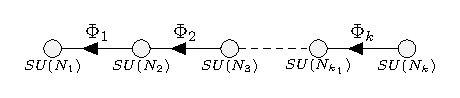
\includegraphics{test.eps}
        \caption{Quiver gauge theory}
        \label{1}
    \end{figure}
\end{frame}

\begin{frame}
    \frametitle{Classification of scattering amplitude}
    For the simplicity, we started front the two-site gauge theory, means that there are only two gauge fields and one scalar field.
    The amplitudes in this theory can be classified to many types
    \begin{columns}[T]
        \begin{column}{0.48\textwidth}
            \begin{itemize}
                \item 3-point
                    \begin{itemize}
                        \item $\bm{V_1\Phi\Phi^\dagger}$
                        \item $\bm{V_2\Phi\Phi^\dagger}$
                        \item $\bm{V_1V_1V_1}$
                        \item $\bm{V_2V_2V_2}$
                    \end{itemize}
            \end{itemize}
        \end{column}
        \begin{column}{0.48\textwidth}
            \begin{itemize}
                \item 4-point
                \begin{itemize}
                    \item $\bm{V_1V_1V_1V_1}$
                    \item $\bm{V_2V_2V_2V_2}$
                    \item $\bm{\Phi^\dagger V_1V_1\Phi}$
                    \item $\bm{\Phi V_2V_2\Phi^\dagger}$
                    \item $\bm{\Phi\Phi^\dagger\Phi\Phi^\dagger}$
                \end{itemize}
            \end{itemize}
        \end{column}
    \end{columns}
\end{frame}



\end{document}